\begin{figure}[!ht]
  \centering
\resizebox{1.01\linewidth}{!} {
  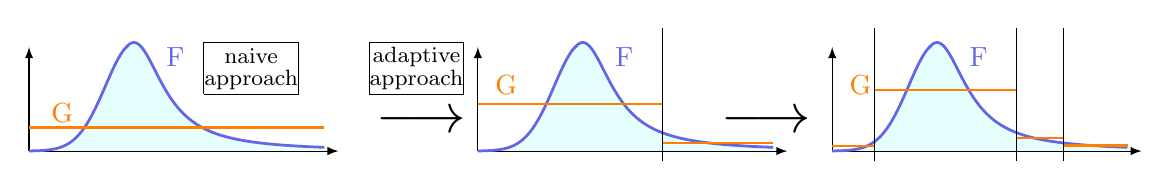
\begin{tikzpicture}[scale=0.6,declare function={
    %%cauchy distrib
    c1 = 6/10;
    c2 = 4/10;
    seuil = c1/(c1+c2);
    a1 = 0.1;
    a2 = 0.2;
    x01 = 0.8;
    x02 = 2.9;
    cauchyMass1(\x) = c1*a1/( pi*( pow(a1,2) + pow((\x-x01),2) ));
    cauchyMass2(\x) = c2*a2/( pi*( pow(a2,2) + pow((\x-x02),2) ));
    loinormale(\x) = c2*exp(-pow((\x-x02),2)/0.05);
    loinormale2(\x) = c2*exp(-pow((\x-x02-1.5),2)/0.3);
      indicatorFunction(\x) = exp(-pow(\x-3,2)/6);
      %%params
      firstVerticalSplitX = 1;
      lastVerticalSplitX = 5.7;
      verticalDashedSplitX = 2.3;
      verticalSplitX = 4;
      lowHorizontalDashedSplitY = 4.5;
      highHorizontalDashedSplitY = 5.5;
      coeffHomothety = 3.8;
      homothetyBone = -1.7;
      homothetyBtwo = -14;
    },
]
  \definecolor{niceblue}{rgb}{0.4,0.4,0.9}
    \definecolor{blue2}{rgb}{0.9,1,1}
\definecolor{ggreen}{rgb}{0.3,0.7,0.4}
\definecolor{orange2}{rgb}{1,0.7,0}

%%%%%%%%%%%%%%%% FIRST curve

\fill [blue2, domain=-7.9:-1.65, variable=\x]
      (-7.9, 1)
      -- plot[samples=200,smooth] ({\x},{ 1.5*coeffHomothety*loinormale((\x-homothetyBone+15)/coeffHomothety)  +1 } )
      -- (-1.47, 1)
      -- cycle;
\fill [blue2, domain=-5.8:-1.65, variable=\x]
      (-5.85, 1)
      -- plot[samples=200,smooth] ({\x},{ 1.5*0.633*coeffHomothety*cauchyMass2((\x-homothetyBone+15)/coeffHomothety)  +1 } )
      -- (-1.47, 1)
      -- cycle;
  \draw[->,>=latex] (-7.9,1) to (-7.9,3.2);
  \draw[->,>=latex] (-7.9,1) to (-1.35,1);
  \draw [domain=-7.9:-5.8, scale=1, color=niceblue, line width=1pt] plot[samples=200,smooth] (\x,{ 1.5*coeffHomothety*loinormale((\x-homothetyBone+15)/coeffHomothety)  +1} );
  \draw [domain=-5.85:-1.65, scale=1, color=niceblue, line width=1pt] plot[samples=200,smooth] (\x,{ 1.5*0.633*coeffHomothety*cauchyMass2((\x-homothetyBone+15)/coeffHomothety)  +1} );

  %% splits
  \draw[color=orange,thick] (-7.9,1.5) -- (-1.65,1.5);

  \node[color=orange] at (-7.2,1.8){G};
  \node[color=niceblue] at (-4.8,3){F};

  \node at (-3.2,3){\footnotesize naive};
  \node at (-3.2,2.5){\footnotesize approach};
  \draw (-4.2,2.2) -- (-2.2,2.2) -- (-2.2,3.3) -- (-4.2,3.3) -- (-4.2,2.2);


\node at (0.3,3){\footnotesize adaptive};
  \node at (0.3,2.5){\footnotesize approach};
  \draw (-0.7,2.2) -- (1.3,2.2) -- (1.3,3.3) -- (-0.7,3.3) -- (-0.7,2.2);
	\node at (0.4,1.6) {\scalebox{2}{$\longrightarrow$}};


%%%%%%%%%%%%%%%% second curve

\fill [blue2, domain=1.6:7.95, variable=\x]
      (1.6, 1)
      -- plot[samples=200,smooth] ({\x},{ 1.5*coeffHomothety*loinormale((\x-homothetyBone+5.5)/coeffHomothety)  +1 } )
      -- (8.03, 1)
      -- cycle;
\fill [blue2, domain=3.65:7.85, variable=\x]
      (3.65, 1)
      -- plot[samples=200,smooth] ({\x},{ 1.5*0.633*coeffHomothety*cauchyMass2((\x-homothetyBone+5.5)/coeffHomothety)  +1 } )
      -- (8.03, 1)
      -- cycle;
  \draw[->,>=latex] (1.6,1) to (1.6,3.2);
  \draw[->,>=latex] (1.6,1) to (8.15,1);
  \draw [domain=1.6:3.7, scale=1, color=niceblue, line width=1pt] plot[samples=200,smooth] (\x,{ 1.5*coeffHomothety*loinormale((\x-homothetyBone+5.5)/coeffHomothety)  +1} );
  \draw [domain=3.65:7.85, scale=1, color=niceblue, line width=1pt] plot[samples=200,smooth] (\x,{ 1.5*0.633*coeffHomothety*cauchyMass2((\x-homothetyBone+5.5)/coeffHomothety)  +1} );


\node[color=niceblue] at (4.7,3){F};


\draw[color=orange,thick] (1.6,2) -- (5.5,2);
\draw[color=orange,thick] (5.5,1.17) -- (7.85,1.17);
	 \node[color=orange] at (2.2,2.4){G};

  %% splits
  \draw (5.5,0.8) -- (5.5,3.6);


  %%%%%%%%%%%%%%%%%% third curve

\fill [blue2, domain=9.1:15.45, variable=\x]
      (9.1, 1)
      -- plot[samples=200,smooth] ({\x},{ 1.5*coeffHomothety*loinormale((\x-homothetyBone-2)/coeffHomothety)  +1 } )
      -- (15.53, 1)
      -- cycle;
\fill [blue2, domain=11.15:15.35, variable=\x]
      (11.15, 1)
      -- plot[samples=200,smooth] ({\x},{ 1.5*0.633*coeffHomothety*cauchyMass2((\x-homothetyBone-2)/coeffHomothety)  +1 } )
      -- (15.53, 1)
      -- cycle;
  \draw[->,>=latex] (9.1,1) to (9.1,3.2);
  \draw[->,>=latex] (9.1,1) to (15.65,1);
  \draw [domain=9.1:11.2, scale=1, color=niceblue, line width=1pt] plot[samples=200,smooth] (\x,{ 1.5*coeffHomothety*loinormale((\x-homothetyBone-2)/coeffHomothety)  +1} );
  \draw [domain=11.15:15.35, scale=1, color=niceblue, line width=1pt] plot[samples=200,smooth] (\x,{ 1.5*0.633*coeffHomothety*cauchyMass2((\x-homothetyBone-2)/coeffHomothety)  +1} );

\node[color=niceblue] at (12.2,3){F};

	\node at (7.7,1.6) {\scalebox{2}{$\longrightarrow$}};

\draw[color=orange,thick] (9.1,1.1) -- (10,1.1);
\draw[color=orange,thick] (10,2.3) -- (13,2.3);
\draw[color=orange,thick] (13,1.28) -- (14,1.28);
\draw[color=orange,thick] (14,1.12) -- (15.35,1.12);
	 \node[color=orange] at (9.7,2.4){G};

  %% splits
  \draw (13,0.8) -- (13,3.6);
\draw (14,0.8) -- (14,3.6);
\draw (10,0.8) -- (10,3.6);

\end{tikzpicture}
}
~\\
 {\small {\blue $F$} is the inliers distribution, {\color{orange} $G$} is the resulting outliers distribution.
% Outliers distribution $G$ in the naive and adaptive approach.  In the naive approach, $G$ does not depends on the tree and is constant on the input space.
% In the adaptive approach $G$ depends on the inlier distribution $F$ through the tree. The outliers density is constant and equal to the average of $F$ on each node before splitting it.
}

  \label{ocrf:fig:outlier_density}
\end{figure}
